\section{2020 年 12 月 13 日答疑记录}

\begin{example}
    求函数 $f(x)=4^x-2^x-2$ 的零点.
\end{example}
\begin{solution}
    令 $f(x)=0$, 则 $4^x-2^x-2=0$, 即
    \[(2^x)^2-2^x-2=0,\quad (2^x-2)(2^x+1)=0.\]
    因为恒有 $2^x>0$, 所以 $2^x=2$, 解得 $x=1$. 故所求零点为 $x=1$. 
\end{solution}

\begin{example}\label{exa:201223-1850}
    设方程 $2^{-x}= |\lg x|$ 的两个根为 $x_1$, $x_2$, 求 $x_1x_2$ 的取值范围.
\end{example}
\begin{solution}
    分别画出函数 $f(x)= 2^{-x}$ 和 $g(x)= |\lg x|$ 的图形, 可知两者交点的横坐标为 $x_1$, $x_2$, 且均为正数并分别在 $1$ 的两侧. 不妨设 $x_1\in(0,1)$, $x_2\in(1,+\infty)$, 由 $f(x)$ 单调递减可知, $f(x_1)>f(x_2)$, 即 $g(x_1)>g(x_2)$, 所以
    \[|\lg x_1|> |\lg x_2|,\quad -\lg x_1> \lg x_2,\]
    整理可得 $\lg (x_1x_2)<0$. 进一步有 $x_1x_2\in(0,1)$.
    
    \begin{center}
        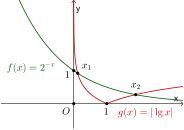
\includegraphics[scale=1]{2020-1223-1900-crop}
    \end{center}
\end{solution}
\begin{remark}
    若将例~\ref{exa:201223-1850} 中的方程改为 $k= |\log_a x|$, 其中 $k$ 为正的常数, $a\in(0,1)\cup (1,+\infty)$, 用同样的方法可以知道 $x_1x_2=1$.
\end{remark}

\begin{example}
    一个容器装有细沙 $a\,\text{cm}^3$, 细沙从容器底部一个细微的小孔慢慢地匀速漏出, $t\,\text{min}$ 后剩余的细沙量为 $y= a\mathrm{e}^{-bt}\,(\text{cm}^3)$, 经过 $8\,\text{min}$ 后发现容器内还有一半的沙子, 求需要再经过多少时间, 容器中的沙子只有开始时的八分之一.
\end{example}
\begin{solution}
    设经过 $t\,\text{min}$ 符合题意, 则由已知,
    \[\left\{\!\!\begin{array}{l}
        a\mathrm{e}^{-b\cdot 8}= \dfrac{a}2,\\[5pt]
        a\mathrm{e}^{-bt}= \dfrac{a}8,
        \end{array}\right.\ \text{即}
      \left\{\!\!\begin{array}{l}
        \mathrm{e}^{-8b}= \dfrac12,\\[3pt]
        \mathrm{e}^{-bt}= \dfrac18.
      \end{array}\right.\]
    因为 $\dfrac18= \biggl(\dfrac12\biggr)^3$, 所以
    \[\mathrm{e}^{-bt}= (\mathrm{e}^{-8b})^3= \mathrm{e}^{-24b},\]
    即 $-bt=-24b$, 解得 $t=24$. 这表明需要再经过 $(t-8)\,\text{min}= 16\,\text{min}$, 才能符合题意.
\end{solution}

\begin{example}
    设函数 $f(x)= \log_{\frac12} x$, 求下列命题中真命题的个数:
    
    (1) 函数 $f(|x|)$ 为偶函数.
    
    (2) 若 $f(a)= |f(b)|$, 其中 $a$, $b>0$ 且 $a\neq b$, 则 $ab=1$.
    
    (3) 函数 $f(-x^2+2x)$ 在 $(1,3)$ 上为单调递增函数.
    
    (4) 若 $0<a<1$, 则 $|f(1+a)|< |f(1-a)|$.   
\end{example}
\begin{solution}
    (1) 设 $g(x)=f(|x|)$, 则 
    \[g(-x)= f(|-x|)= f(|x|)= g(x),\]
    所以函数 $f(|x|)$ 为偶函数 (此结论无需考虑 $f(x)$ 的具体表达式).
    
    (2) $f(x)= |f(b)|$ 化为 $\log_{\frac12} a= |\log_{\frac12} b|$, 由此可知 $\log_{\frac12} a\geqslant 0$, 即 $a\in(0,1]$. 若 $b\in(0,1]$, 则 $\log_{\frac12} a= \log_{\frac12} b$, 必有 $a=b$, 与已知矛盾. 若 $b\in(1,+\infty)$, 则 
    \[\log_{\frac12} a= -\log_{\frac12} b,\quad\text{即}\quad
        \log_{\frac12} ab=0,\]
    所以 $ab=1$.
    
    (3) 函数 $f(-x^2+2x)= \log_{\frac12}(-x^2+2x)$, 定义域为 $(0,2)$, 所以在 $(1,3)$ 并非处处有定义, 无法判断定义域. (如果只考虑 $x\in(1,2)$, 则可由复合函数的单调性知, 函数 $f(-x^2+2x)$ 为单调递增函数.)
    
    (4) 方法一: 因为 $0<a<1$, 所以 $1-a\in(0,1)$, $1+a\in(1,2)$,
    \[\begin{aligned}
        |f(1+a)|- |f(1-a)|
        &= |\log_{\frac12} (1+a)|- |\log_{\frac12} (1-a)|\\
        &= -\log_{\frac12} (1+a)- \log_{\frac12} (1-a)\\
        &= -\log_{\frac12} (1-a^2)<0,
    \end{aligned}\] 
    即 $|f(1+a)|- |f(1-a)|<0$, 因此 $|f(1+a)|< |f(1-a)|$.
    
    方法二: 直接画函数 $h(x)= |\log_{\frac12} x|$ 的图形, 并由图形单调性可知,
    \[|f(1+a)|< |f(1-a)|.\]
    
    \begin{center}
        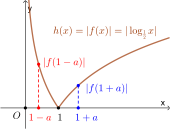
\includegraphics[scale=1]{2020-1223-1940-crop}
    \end{center}
    
    综上所述, (1)(2)(4) 是真命题, 共 $3$ 个.
\end{solution}

\begin{example}
    已知函数 $f(x)= \dfrac{2x+1}{x+1}$, 求该函数在区间 $[1,4]$ 上的最大值与最小值.
\end{example}
\begin{solution}
    用分离常数法, 
    \[f(x)= \frac{2x+1}{x+1}= \frac{2(x+1)-1}{x+1}
        = 2-\frac1{x+1}.\]
    因为 $x\in[1,4]$, 所以 $\dfrac1{x+1}$ 单调递减, $-\dfrac1{x+1}$ 单调递增, $2-\dfrac1{x+1}$ 也单调递增, 从而 
    \[f_{\min}= f(1)= \dfrac32,\quad f_{\max}= f(4)= \dfrac95.\]
\end{solution}

\begin{example}
    大气中的温度随着高度的上升而降低, 根据实测的结果, 上升到 $12\,\text{km}$ 为止温度的降低大体上与升高的距离成正比, 在 $12\,\text{km}$ 以上温度一定, 保持在 $-55\,\textcelsius$.
    
    (1) 当地表大气的温度是 $a\,\textcelsius$ 时, 在 $x\,\text{km}$ 上空的温度为 $y\,\textcelsius$, 求 $a$, $x$, $y$ 之间的函数关系式;
    
    (2) 当地表大气的温度是 $29\,\textcelsius$ 时, 在 $3\,\text{km}$ 上空的温度是多少?
\end{example}
\begin{solution}
    (1) 设题中的正比例系数为 $k$, 则 $a-y=kx$. 因为当 $x=12$ 时, $y=-55$, 所以 
    \[a-(-55)= k\cdot 12,\quad\text{即}\quad
        k= \frac{a+55}{12}.\]
    进一步可得,
    \[y=\begin{cases}
        a-\dfrac{a+55}{12}, & x\in[0,12],\\
        -55, & x\in(12,+\infty).
    \end{cases}\]
    
    (2) 此时 $a=29$, 当 $x=3$ 时, $y=29 -\dfrac{29+55}{12}=22$.
\end{solution}

\begin{example}
    已知函数 $f(x)= \log_a (2-x)+\log_a(x+2)$ 的最小值为 $-4$, 其中 $0<a<1$, 求 $a$ 的值.
\end{example}
\begin{solution}
    由题意,
    \[\left\{\!\!\begin{array}{l}
        2-x>0,\\
        x+2>0,
      \end{array}\right.\ \text{解得}\quad x\in(-2,2).\]
    因为 $f(x)= \log_a (4-x^2)$, 而 $4-x^2\in(0,4]$, 所以由 $\log_a x$ 单调递减可知, $f(x)\in[\log_a 4,+\infty)$. 因此 
    \[\log_a 4=-4,\quad a^{-4}= 4,\quad
        a= 4^{-\frac14}= \frac{\sqrt2}2.\]
\end{solution}

\begin{example}
    已知 $\log_a \dfrac23<1$, 求实数 $a$ 的取值范围.
\end{example}
\begin{solution}
    不等式化为 $\log_a \dfrac23< \log_a a$.

    (1) 若 $a\in(0,1)$, 由 $\log_a x$ 单调递减可知, $a<\dfrac23$, 所以 $a\in\biggl(0,\dfrac23\biggr)$.
    
    (2) 若 $a\in(1,+\infty)$, 由 $\log_a x$ 单调递增可知, $a>\dfrac23$, 所以 $a\in(1,+\infty)$.
    
    综上所述, $a\in\biggl(0,\dfrac23\biggr)\cup(1,+\infty)$.
\end{solution}

\begin{example}
    若函数 $y= 2^{|x-1|}$ 在区间 $(k-1,k+1)$ 内不单调, 求 $k$ 的取值范围.
\end{example}
\begin{solution}
    由 $y=2^|x|$ 的图形向右平移一个单位长度可得 $y= 2^{|x-1|}$ 的图形, 而前者为偶函数, 且当 $x\geqslant 0$ 时 $y=2^x$. 由此可以画出 $y= 2^{|x-1|}$ 的图形如下:
    
    \begin{center}
        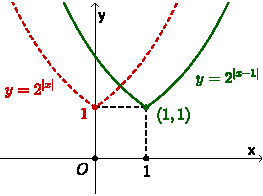
\includegraphics[scale=1]{2020-1223-2000-crop}
    \end{center}
    
    由图可知, $y= 2^{|x-1|}$ 在 $(-\infty,1)$ 上单调递减, 在 $(1,+\infty)$ 上单调递增. 因为题中要求函数 $y= 2^{|x-1|}$ 在区间 $(k-1,k+1)$ 内不单调, 所以
    \[1\in(k-1,k+1),\quad\text{解得}\quad k\in(0,2).\]
\end{solution}